\section{Early Classification of Time Series}
\label{sec:early}

Early classification of time series is the task of performing a classification
as early as possible for an incoming time series.
% Because of the specificity of this task, I will use in this section the
% notation $\mathbf{x}_{\rightarrow t}$ to denote the time series $\mathbf{x}$
% truncated after $t$ timestamps.

I have worked on two methods for this task.
The first one is a slight improvement
over~\cite{dachraoui2015early} and the second one relies on a
representation-learning strategy.

\subsection{Optimizing a Composite Loss for Early Classification}

\cite{dachraoui2015early} introduces a composite loss function for early
classification of time series that balances earliness and accuracy.

The cost function is of the following form:

\begin{equation}
\mathcal{L}(\mathbf{x}_{\rightarrow t}, y, t, \boldsymbol{\theta}) =
    \mathcal{L}_c(\mathbf{x}_{\rightarrow t}, y, \boldsymbol{\theta}) + \alpha t
\label{eq:loss_early}
\end{equation}

\noindent
where $\mathcal{L}_c(\cdot,\cdot,\cdot)$ is a
classification loss and $t$ is the time at which a
decision is triggered by the system.
In this setting, $\alpha$ drives the tradeoff between accuracy and earliness
and is supposed to be a hyper-parameter of the method.

The authors rely on (i) a clustering of the
training
time series and (ii) individual classifiers $m_t(\cdot)$ trained at all possible
timestamps, so as to be able to predict, at time $t$, an expected cost for all
times $t + \tau$ with $\tau \geq 0$:

\begin{equation}
    f_\tau(\mathbf{x}_{\rightarrow t}, y) =
        \sum_k \left[ P(C_k | \mathbf{x}_{\rightarrow t})
        \sum_i \left( P(y=i | C_k)
        \left( \sum_{j \neq i} P_{t+\tau}(\hat{y} = j | y=i, C_k)
        \right) \right)
        \right]
        + \alpha t
        \label{eq:dachraoui}
\end{equation}

where:

\begin{itemize}
\item $P(C_k | \mathbf{x}_{\rightarrow t})$ is a soft-assignment weight of
$\mathbf{x}_{\rightarrow t}$ to cluster $C_k$;
\item $P(y=i | C_k)$ is obtained from a contingency table that stores the number of
training time series of each class in each cluster;
\item $P_{t+\tau}(\hat{y} = j | y=i, C_k)$ is obtained through training time
confusion matrices built on time series from cluster $C_k$ using classifier
$m_{t+\tau}(\cdot)$.
\end{itemize}

At test time, if a series is observed up to time $t$ and if, for all positive
$\tau$ we have
$f_\tau(\mathbf{x}_{\rightarrow t}, y) \geq f_0(\mathbf{x}_{\rightarrow t}, y)$,
then a decision is made using classifier $m_t(\cdot)$.

\subsubsection{Limitations of the Clustering}

Relying on Equation \eqref{eq:dachraoui} to decide prediction time can be
tricky. We show in the following that in some cases (related to specific
configurations of the training time confusion matrices), such an approach will
lead to undesirable behaviors.%
\footnote{This unpublished note is part of François Painblanc's PhD work.
We are co-supervising François together with Laetitia Chapel and Chloé Friguet.}

Using Bayes' rule, Equation \eqref{eq:dachraoui} can be re-written

\begin{eqnarray}
    f_\tau(\mathbf{x}_{\rightarrow t}, y) &=&
        \sum_k P(C_k | \mathbf{x}_{\rightarrow t})
        \sum_i
        \sum_{j \neq i} P_{t+\tau}(\hat{y} = j, y=i | C_k)
        + \alpha t \\
    &=&
        \sum_k P(C_k | \mathbf{x}_{\rightarrow t})
        \underbrace{\sum_i 1 - P_{t+\tau}(\hat{y} = i, y=i | C_k)}_{A_{t+\tau}(C_k)}
        + \alpha t
\end{eqnarray}

where $A_{t+\tau}(C_k)$ is the sum of off-diagonal elements in the (normalized)
training time confusion matrix built from time series in cluster $k$ using
classifier $m_{t+\tau}(\cdot)$.

In practice, this means that if the sum of off-diagonal elements of confusion
matrices is equal to the same $A_{t+\tau}$ for all clusters, then this method
will make a decision on the most adequate prediction time without taking the
data $\mathbf{x}_{\rightarrow t}$ into account:

\begin{eqnarray}
    f_\tau(\mathbf{x}_{\rightarrow t}, y) &=&
        \sum_k P(C_k | \mathbf{x}_{\rightarrow t})
        A_{t+\tau}
        + \alpha t \\
     &=&
        A_{t+\tau} + \alpha t
\end{eqnarray}

In other words, for this method to adapt the decision time $t$ in a
data-dependent fashion, it is important that accuracy differs
significantly between clusters, which is a condition that is difficult to ensure
\emph{a priori}.

\subsection{Pushing the Method to the Limit Case}

In~\cite{tavenard:halshs-01339007}, we pushed this method to its limit case
where the number of clusters is equal to the number of training time series.
In this case, the limitation exposed above does not hold anymore.

We showed superior loss optimization capabilities with this approach, at the
cost of a larger computational complexity.

We also showed that in order to limit inference time complexity, one could
learn a \emph{decision triggering classifier} that, based on the time series
$\mathbf{x}_{\rightarrow t}$, predicts whether a decision should be triggered
or not.
In this setting, the target values $\gamma_t$ used to train this
\emph{decision triggering classifier}
were computed from expected costs $f_\tau$ presented above:

\begin{equation}
    \gamma_t(\mathbf{x}_{\rightarrow t}, y) = \left\{
        \begin{array}{l}
            1 \text{ if } f_{0}(\mathbf{x}_{\rightarrow t}, y) =
                \min_{\tau \geq 0} f_{\tau}(\mathbf{x}_{\rightarrow t}, y) \\
            0 \text{ otherwise. }
        \end{array} \right.
\end{equation}

In other words, decision making is here seen as a two-step process where a
first classifier (\emph{decision triggering classifier}) decides whether a decision
should be made, in which case a
second classifier is used to determine the class to be predicted (the latter
classifier is $m_t(\cdot)$, the same as for other methods).

\subsection{Representation Learning for Early Classification}

The previous approach has several shortcomings.
First, it requires to learn a classifier $m_t(\cdot)$ for each possible time
series length $t$, which is very costly.
Second, both classifiers (the one that decides whether a decision should be
made, and the one that actually makes the decision) are seen as independent
models, while they are, in practice, closely related.
Finally, the loss function presented in Equation \eqref{eq:loss_early} requires
a careful choice of hyper-parameter $\alpha$ that might not be easy to
determine in
practice.%
\footnote{This work is part of Marc Rußwurm's PhD work.
Marc is a PhD student from TU Munich who came to France for a
4-month period in 2018-2019. I was co-supervising Marc with Nicolas Courty
and Sébastien Lefèvre during his stay.}

We have hence proposed a representation learning framework that
addresses these three limitations~\cite{ruwurm:hal-02174314}.

In more detail, we rely on a feature extraction module (that can either be
made of causal convolutions or recurrent submodules) to extract a fixed-sized
representation $h_t$ from an incoming time series $\mathbf{x}_{\rightarrow t}$.
An important point here is that this feature extractor should operate on time
series whatever their length (and hence a different feature extractor need not
to be learned for each time series length).
Then, this feature is provided as input to two different heads, as shown in
Figure~\ref{fig:early}.

\begin{figure}[t]
\centering
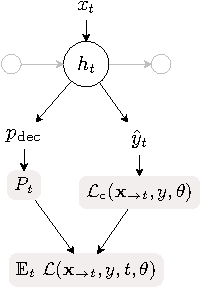
\includegraphics[width=.3\textwidth]{fig/early_module_cropped}
\caption{End-to-end differentiable early classification model.
Grey cells correspond to quantities that are
computed from the model outputs. \label{fig:early}}
\end{figure}

\begin{itemize}
\item The first head (left) outputs a probability $p_\text{dec}$ of making a
decision at
time $t$ given that no decision has been made before: it plays the same role
as the \emph{decision triggering classifier} presented above and from the series of
$p_\text{dec}$ values, one can compute the probability $P_t$ of making a
decision at time $t$;
\item The second head is the standard classification head that effectively produces
a classification if the first head triggered it.
\end{itemize}

Hence, provided that we have a differentiable early classification loss
function, we are able to learn all parameters of this model end-to-end.
Our last contribution in this context is the design of a loss function that
does not lead to dumb optimal solutions (\emph{e.g.}, trigger all
classifications at
the first time stamp, whatever the data).
We introduced the following loss function:

\begin{equation}
    \mathcal{L}(\mathbf{x}_{\rightarrow t}, y, t, \boldsymbol{\theta}) =
        \alpha \mathcal{L}_c(\mathbf{x}_{\rightarrow t}, y, \boldsymbol{\theta})
            - (1-\alpha) P_{\boldsymbol{\theta}}(m_t(\mathbf{x}_{\rightarrow t})=y)
            \left( \frac{T-t}{T} \right)
\end{equation}

\noindent
where $P_{\boldsymbol{\theta}}(m_t(\mathbf{x}_{\rightarrow t})=y)$ is the
probability (as
assigned by the classification model) to generate $y$ as an output and $T$ is
the total length of the time series (\emph{i.e.} the maximum timestamp at which
a decision can be made).
The second part in this loss function is an earliness reward, which is taken
into account iff the provided decision is sound (\emph{i.e.} the correct class
is
predicted with non-zero probability).
When the decision time is drawn from the
multinomial distribution of parameters $\{P_t\}_{t \in [0, T-1]}$, the overall
loss is now:
\begin{equation}
    \mathbb{E}_{t \sim \mathcal{M}(P_0, \dots , P_{T-1})}
        \mathcal{L}(\mathbf{x}_{\rightarrow t}, y, t, \boldsymbol{\theta})
\end{equation}
and gradients can be back-propagated through both heads of the model, hence
allowing to jointly learn the early decision mechanism and the predictor.

We have shown that this model outperforms all known baselines in terms of both
time complexity and earliness/accuracy tradeoff, especially for large scale
datasets.
Moreover, we have presented an application of this model to the monitoring of
agriculture, and demonstrated its ability to trigger class-specific early
decisions in this context in~\cite{ruwurm:hal-02343851}.
